\documentclass[11pt,letterpaper]{article}
\usepackage{xcolor}
\usepackage{textcomp,marvosym}
\usepackage{amsmath,amssymb}
\usepackage[left]{lineno}
\usepackage{changepage}
\usepackage{rotating}
\usepackage{natbib}
\usepackage{setspace}
\usepackage{fancyhdr}
\usepackage{graphicx}
\usepackage{sidecap}
\usepackage{pdfpages}
\usepackage{longtable}

\usepackage[aboveskip=1pt,labelfont=bf,labelsep=period,justification=raggedright,singlelinecheck=off]{caption}
%\doublespacing

\raggedright
\textwidth = 6.5 in
\textheight = 8.25 in
\oddsidemargin = 0.0 in
\evensidemargin = 0.0 in
\topmargin = 0.0 in
\headheight = 0.0 in
\headsep = 0.5 in
\parskip = 0.0 in
\parindent = 0.2 in

\pagestyle{myheadings}
\pagestyle{fancy}
\fancyhf{}
\lhead{Data Repository (Rapid emplacement of massive Duluth Complex intrusions)}
\rhead{\thepage}

\begin{document}

\subsection*{Data repository materials for ``Rapid emplacement of massive Duluth Complex intrusions within the Midcontinent Rift''}

\renewcommand{\thefigure}{DR\arabic{figure}}
\begin{figure}[!ht]
\noindent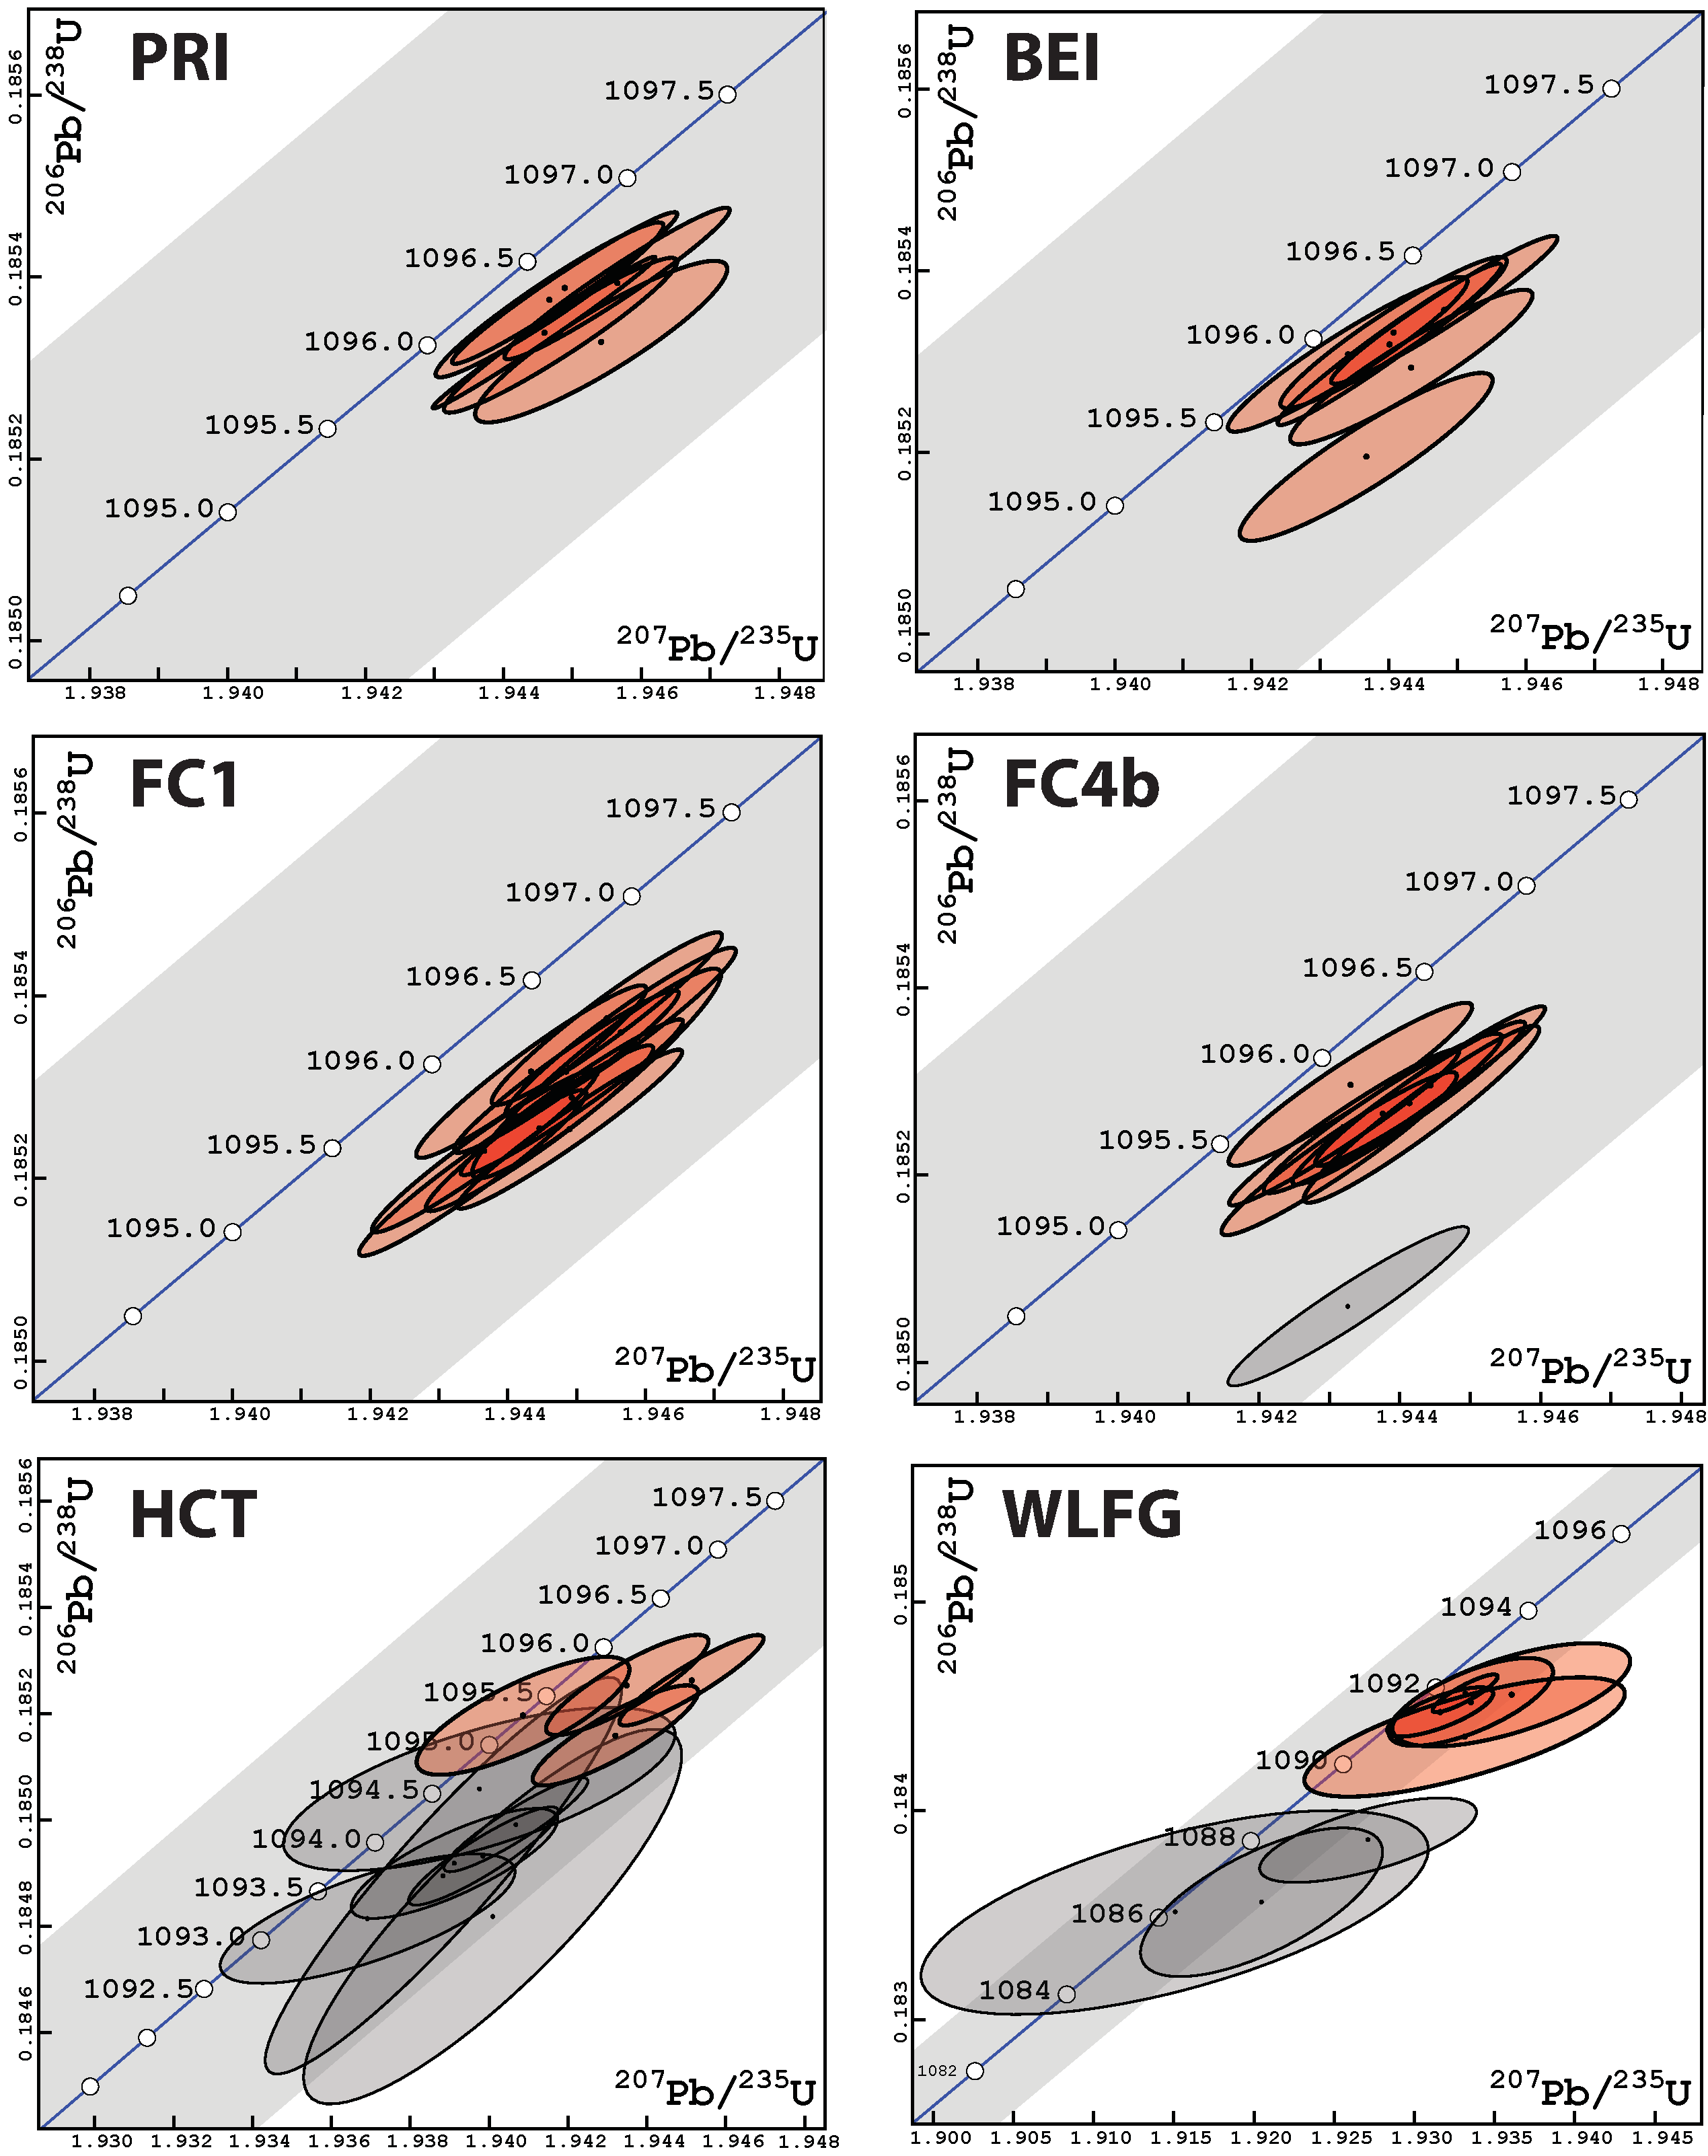
\includegraphics[width=0.8\textwidth]{./repository/Concordia_Plots.pdf}
\centering
\caption{\small{U-Pb concordia plots for the new zircon dates. The grey region illustrates uncertainty on concordia due to the decay constant uncertainties. The ellipses represent  2$\sigma$ analytical uncertainty on individual zircon dates. Red ellipses are analyses included in the $^{206}$Pb/$^{238}$U weighted mean dates while the grey ellipses are those that were excluded. The scale is the same for the PRI, BEI, FC1 and FC4b data and zoomed out for HCT and WLFG as a result of grains that we interpret to have unmitigated Pb loss.}}
\label{fig:map}
\end{figure}

\subsubsection*{CA-TIMS U-Pb Geochronology Methods}

{\footnotesize\textcolor{red}{This method section needs to be reviewed by Mark in consultation with the data reduction files. A note from Jim in this regard says: ``\textit{There are several things I do not know because Mark did the data reduction. One is the U ratio. I put in 137.88. Other is how the Th-U disequilibrium correction was done. This should make little difference for samples this old, but we should still ask Mark to make sure we get it correct. Final thing is whether any of the analyses had enough radiogenic Pb so that the Pb was run on the Faraday cups instead of the Daly.}''}}

U-Pb dates were obtained by the chemical abrasion isotope dilution thermal ionization mass spectrometry (CA-TIMS) method from analyses composed of single zircon grains (Table DR1), modified after \cite{Mattinson2005a}. Zircon was separated from rocks using standard techniques, and placed in a muffle furnace at 900\textdegree C for 60 hours in quartz beakers.

Zircon was put into 3 ml Teflon PFA beakers and loaded into 300 $\mu$l Teflon PFA microcapsules. Fifteen microcapsules were placed in a large-capacity Parr vessel and the zircon partially dissolved in 120 $\mu$l of 29 M HF for 12 hours at 180\textdegree C. Zircon was returned to 3 ml Teflon PFA beakers, HF was removed, and zircon was immersed in 3.5 M HNO$_\mathrm{3}$, ultrasonically cleaned for an hour, and fluxed on a hotplate at 80\textdegree C for an hour. The HNO$_\mathrm{3}$ was removed and zircon was rinsed twice in ultrapure H$_\mathrm{2}$O before being reloaded into the 300 $\mu$l Teflon PFA microcapsules (rinsed and fluxed in 6 M HCl during sonication and washing of the zircon) and spiked with the EARTHTIME mixed $^{233}$U-$^{235}$U-$^{205}$Pb tracer solution (ET535). Zircon was dissolved in Parr vessels in 120 $\mu$l of 29 M HF with a trace of 3.5 M HNO$_\mathrm{3}$ at 220\textdegree C for 48 hours, dried to fluorides, and re-dissolved in 6 M HCl at 180\textdegree C overnight. U and Pb were separated from the zircon matrix using an HCl-based anion-exchange chromatographic procedure \citep{Krogh1973a}, eluted together and dried with 2 $\mu$l of 0.05 N H$_\mathrm{3}$PO$_\mathrm{4}$.

Pb and U were loaded on a single outgassed Re filament in 5 $\mu$l of a silica-gel/phosphoric acid mixture \citep{Gerstenberger1997a}, and U and Pb isotopic measurements made on a GV Isoprobe-T multicollector thermal ionization mass spectrometer equipped with an ion-counting Daly detector. Pb isotopes were measured by peak-jumping all isotopes on the Daly detector for 160 cycles, and corrected for 0.16 $\pm$ 0.03$\%$/a.m.u. (1$\sigma$) mass fractionation. Transitory isobaric interferences due to high-molecular weight organics, particularly on $^{204}$Pb and $^{207}$Pb, disappeared within approximately 30 cycles, while ionization efficiency averaged 10$^4$ cps/pg of each Pb isotope. Linearity (to $\geq$1.4 x 10$^6$ cps) and the associated deadtime correction of the Daly detector were determined by analysis of NBS982. Uranium was analyzed as UO$_2^+$ ions in static Faraday mode on 10$^{11}$ ohm resistors for 300 cycles, and corrected for isobaric interference of $^{233}$U$^{18}$O$^{16}$O on $^{235}$U$^{16}$O$^{16}$O with an $^{18}$O/$^{16}$O of 0.00206. Ionization efficiency averaged 20 mV/ng of each U isotope. U mass fractionation was corrected using the known $^{233}$U/$^{235}$U ratio of the ET535 tracer solution.

CA-TIMS U-Pb dates and uncertainties were calculated using the algorithms of \cite{Schmitz2007a}, ET535 tracer solution \cite{Condon2015a} with calibration of $^{235}$U/$^{205}$Pb = 100.233, $^{233}$U/$^{235}$U = 0.99506, and $^{205}$Pb/$^{204}$Pb = 11268, and U decay constants recommended by \cite{Jaffey1971a}, including $^{238U}$/$^{235}$U of 137.88. $^{206}$Pb/$^{238}$U ratios and dates were corrected for initial $^{230}$Th disequilibrium using D$_{Th/U}$ = 0.2 $\pm$ 0.1 (2$\sigma$) and the algorithms of \cite{Crowley2007a}, resulting in an increase in the $^{206}$Pb/$^{238}$U dates of $\sim$0.09 Ma. All common Pb in analyses was attributed to laboratory blank and subtracted based on the measured laboratory Pb isotopic composition and associated uncertainty. U blanks are estimated at 0.013 pg.

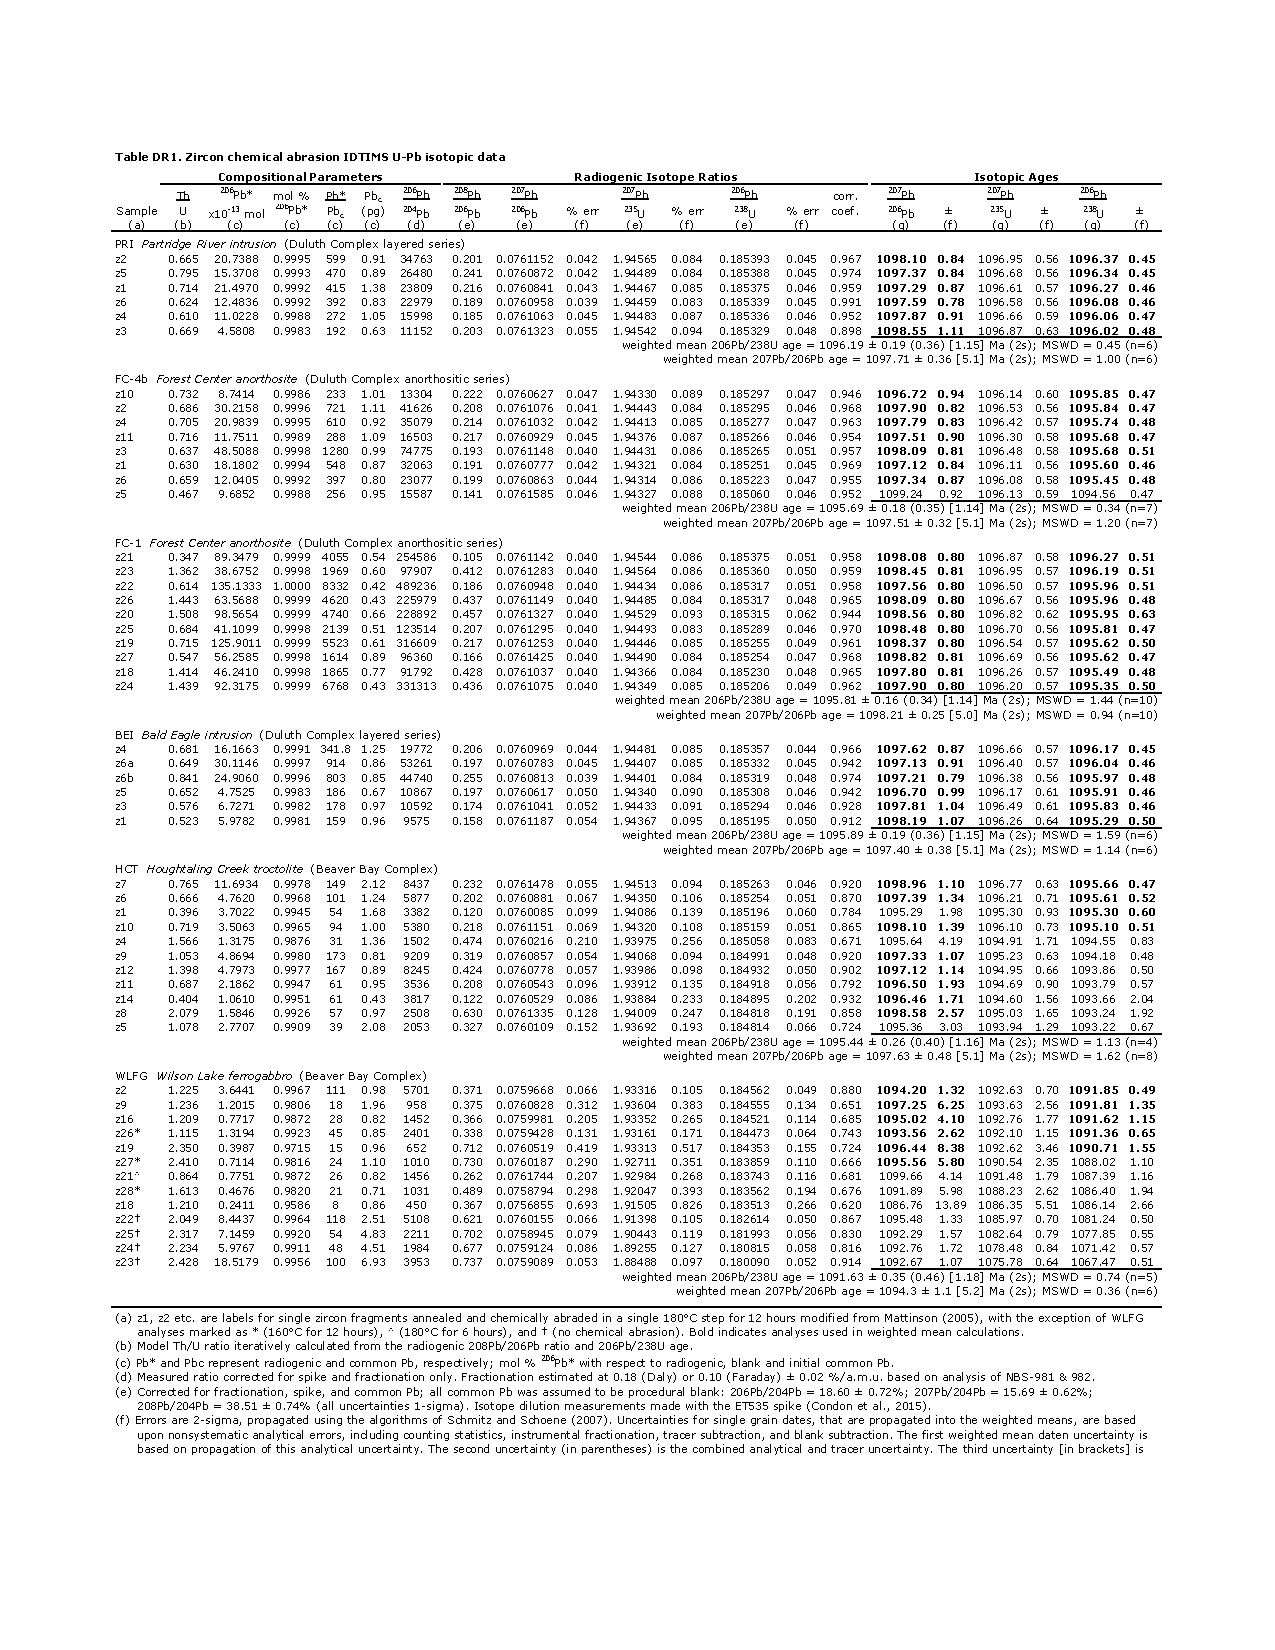
\includepdf[pages=-,pagecommand={},width=8 in]{repository/Repository_Geochronology_Table.pdf}

%\renewcommand{\thetable}{DR\arabic{table}}
%\addtocounter{table}{1}
%\begin{table}[h!]
%\footnotesize
%\caption{$^{207}$Pb/$^{206}$Pb dates for the Midcontinent Rift intrusion dates discussed in the paper}
%\begin{tabular}{|p{3 cm}|p{3.4 cm}|p{3.4 cm}|cc|c|c|}
%\hline
%Sample & $^{207}$Pb/$^{206}$Pb date (Ma) & $^{207}$Pb/$^{206}$Pb date (Ma) & \multicolumn{2}{|c|}{Uncertainty (2$\sigma$)} & MSWD & n/N \\
% &  $^{238}$U/$^{235}$U = 137.818 & $^{238}$U/$^{235}$U = 137.88 & X & Z & & \\
%  &  \cite{Hiess2012a} & \cite{Steiger1977a} &  & & & \\
%\hline
%PRI \textit{Partridge River intrusion}  & & 1097.73  & 0.36 & 5.1 & 0.99 & 6/6 \\
%\hline
%BEI \textit{Bald Eagle intrusion} &  & 1097.40 & 0.38 & 5.1 & 1.14 & 6/6 \\
%\hline
%AS3 \textit{Duluth anorthosite} &  &  1098.59 & 0.33 & 5.1 & 0.37 & 8/8 \\
%\hline
%FC1 \textit{Forest Center anorthosite}   & & 1098.21 & 0.25 & 5.0 & 0.94 & 10/10 \\
%\hline
%FC4b \textit{Forest Center anorthosite}   &  & 1097.53 & 0.32 & 5.1 & 1.20 & 7/8 \\
%\hline
%HCT \textit{Houghtaling Creek troctolite}   & & 1097.43 & 0.46 & 5.1 & 1.93 & 11/11 \\
%\hline
%WLFG \textit{Wilson Lake ferrogabbro}   & & 1094.2 & 1.1 & 5.1 & 0.51 & 8/8 \\
%\hline
%BBC-SBA1 \textit{Silver Bay aplite}  &  1093.22 & 1094.15 & 0.51 &5.1 & 0.86 & 6/6 \\
%\hline
%\end{tabular}\\
%%\begin{tablenotes}[para,flushleft]
%\textcolor{red}{What U ratio are the 7/6 dates in the table using? Are these means in the right columns?}
%Notes: X--internal (analytical) uncertainty in the absence of external or systematic uncertainties; Z--uncertainty including X, as well as decay constant uncertainty \citep{Jaffey1971a}). This Z uncertainty needs to be utilized when comparing to dates developed using other decay systems (e.g., $^{40}$Ar/$^{39}$Ar, $^{187}$Re-$^{187}$Os); MSWD--mean square of weighted deviates; n--number of individual zircon dates included in the calculated sample mean date; N--number of individual zircons analyzed for the sample. All dates are from this study with the exceptions of AS3 which was published in \cite{Schoene2006a} and BBC-SBA1 which was published in \cite{Fairchild2017a}. Data for individual zircons are provided in the Data Repository.
%%\end{tablenotes}
%\label{tab:geochron}
%\end{table}

\renewcommand{\thetable}{DR\arabic{table}}
\addtocounter{table}{1}
\begin{table}[h!]
\footnotesize
\caption{$^{207}$Pb/$^{206}$Pb dates for the Midcontinent Rift intrusion dates discussed in the paper using the \cite{Steiger1977a} $^{238}$U/$^{235}$U ratio of 137.88 for comparison to previously published dates {\footnotesize\textcolor{red}{should we include this table?}}}
\begin{tabular}{|p{3 cm}|p{3.4 cm}|p{3.4 cm}|cc|c|c|}
\hline
Sample & $^{207}$Pb/$^{206}$Pb date (Ma) & $^{207}$Pb/$^{206}$Pb date (Ma) & \multicolumn{2}{|c|}{Uncertainty (2$\sigma$)} & MSWD & n/N \\
 &  $^{238}$U/$^{235}$U = 137.818 & $^{238}$U/$^{235}$U = 137.88 & X & Z & & \\
  &  \cite{Hiess2012a} & \cite{Steiger1977a} &  & & & \\
\hline
PRI \textit{Partridge River intrusion}  & & 1097.73  & 0.36 & 5.1 & 0.99 & 6/6 \\
\hline
BEI \textit{Bald Eagle intrusion} &  & 1097.40 & 0.38 & 5.1 & 1.14 & 6/6 \\
\hline
AS3 \textit{Duluth anorthosite} &  &  1098.59 & 0.33 & 5.1 & 0.37 & 8/8 \\
\hline
FC1 \textit{Forest Center anorthosite}   & & 1098.21 & 0.25 & 5.0 & 0.94 & 10/10 \\
\hline
FC4b \textit{Forest Center anorthosite}   &  & 1097.53 & 0.32 & 5.1 & 1.20 & 7/8 \\
\hline
HCT \textit{Houghtaling Creek troctolite}   & & 1097.43 & 0.46 & 5.1 & 1.93 & 11/11 \\
\hline
WLFG \textit{Wilson Lake ferrogabbro}   & & 1094.2 & 1.1 & 5.1 & 0.51 & 8/8 \\
\hline
BBC-SBA1 \textit{Silver Bay aplite}  &  1093.22 & 1094.15 & 0.51 &5.1 & 0.86 & 6/6 \\
\hline
\end{tabular}\\
%\begin{tablenotes}[para,flushleft]
\textcolor{red}{I think that the U ratio of the 7/6 dates in the table are using 137.88. This needs to be confirmed with Mark and added to the DR1 table notes. Should we provide dates using the updated ratio in this table as well?}
Notes: X--internal (analytical) uncertainty in the absence of external or systematic uncertainties; Z--uncertainty including X, as well as decay constant uncertainty \citep{Jaffey1971a}). This Z uncertainty needs to be utilized when comparing to dates developed using other decay systems (e.g., $^{40}$Ar/$^{39}$Ar, $^{187}$Re-$^{187}$Os); MSWD--mean square of weighted deviates; n--number of individual zircon dates included in the calculated sample mean date; N--number of individual zircons analyzed for the sample. All dates are from this study with the exceptions of AS3 which was published in \cite{Schoene2006a} and BBC-SBA1 which was published in \cite{Fairchild2017a}. Data for individual zircons are provided in the Data Repository.
%\end{tablenotes}
\label{tab:geochron}
\end{table}


\begin{table}[h!]
\tiny
\caption{Site level paleomagnetic data}
\begin{tabular}{|l|r|r|r|r|r|r|r|r|r|r|r|}
\hline
site & site lat & site lon & n & dec$_{is}$ & inc$_{is}$ & dec$_{tc}$ & inc$_{tc}$ & k & $\alpha_{95}$ & VGP lat & VGP lon \\
\hline
	FC1 (AF)		&	47.7826	&	-91.3265	&	9	&	301.6	&	40.5	&	297.1	&	52.4	&	32	&	9.3	&	41.3	&	185.0	\\
\textbf{FC1 (thermal)	}	&	47.7826	&	-91.3265	&	9	&	289.7	&	34.4	&	284.1	&	45.1	&	64	&	6.5	&	28.6	&	187.8	\\
\textbf{FC4 (AF)	}	&	47.7625	&	-91.3827	&	7	&	296.0	&	26.8	&	292.6	&	38.3	&	59	&	7.9	&	30.8	&	177.4	\\
	HCT1 (AF)		&	47.6008	&	-91.1495	&	7	&	287.2	&	35.6	&	281.0	&	46.0	&	54	&	8.3	&	26.9	&	190.8	\\
\textbf{HCT1 (thermal)	}	&	47.6008	&	-91.1495	&	6	&	285.7	&	45.3	&	276.3	&	55.3	&	144	&	5.6	&	29.5	&	201.0	\\
\textbf{1 (Beck layered)	}	&	46.68	&	-92.24	&	4	&	279.5	&	47.5	&	287.7	&	64.4	&	51	&	9.8	&	42.0	&	205.2	\\
	3 (Beck layered)		&	46.68	&	-92.24	&	4	&	292.0	&	26.5	&	298.0	&	41.9	&	17	&	17.2	&	36.3	&	175.6	\\
	4 (Beck layered)		&	46.68	&	-92.24	&	3	&	279.5	&	36.0	&	284.5	&	53.0	&	20	&	18.0	&	33.0	&	193.5	\\
	5 (Beck layered)		&	46.68	&	-92.24	&	3	&	279.5	&	55.0	&	291.8	&	71.7	&	14	&	22.0	&	48.4	&	217.4	\\
	6 (Beck layered)		&	46.68	&	-92.24	&	1	&	280.5	&	32.0	&	285.0	&	48.9	&		&		&	31.1	&	189.7	\\
\textbf{7 (Beck layered)	}	&	46.68	&	-92.24	&	5	&	278.0	&	33.0	&	282.0	&	50.1	&	85	&	6.8	&	29.7	&	192.7	\\
\textbf{8 (Beck layered)	}	&	46.68	&	-92.24	&	7	&	290.5	&	43.0	&	301.6	&	58.3	&	345	&	2.8	&	47.5	&	189.4	\\
\textbf{9 (Beck layered)	}	&	46.68	&	-92.23	&	3	&	281.5	&	42.0	&	288.7	&	58.7	&	35	&	13.6	&	39.2	&	197.0	\\
	10 (Beck layered)		&	46.70	&	-92.23	&	3	&	297.5	&	30.5	&	305.6	&	44.9	&	15	&	21.2	&	43.0	&	172.0	\\
	11 (Beck layered)		&	46.70	&	-92.22	&	1	&	284.0	&	30.5	&	289.2	&	47.0	&		&		&	32.9	&	185.6	\\
\textbf{12 (Beck layered)	}	&	46.72	&	-92.21	&	5	&	284.5	&	36.0	&	291.1	&	52.4	&	43	&	9.6	&	37.1	&	188.9	\\
\textbf{13 (Beck layered)	}	&	46.69	&	-92.24	&	6	&	281.5	&	28.0	&	285.6	&	44.8	&	437	&	2.7	&	29.3	&	186.4	\\
\textbf{14 (Beck layered)	}	&	46.72	&	-92.20	&	7	&	287.0	&	35.0	&	294.1	&	51.1	&	334	&	2.9	&	38.4	&	185.8	\\
	15 (Beck layered)		&	46.73	&	-92.21	&	2	&	290.0	&	31.5	&	296.9	&	47.2	&		&		&	38.2	&	180.4	\\
\textbf{17 (Beck layered)	}	&	46.74	&	-92.19	&	3	&	279.5	&	37.0	&	284.7	&	54.0	&	80	&	9.1	&	33.8	&	194.3	\\
\textbf{19 (Beck layered)	}	&	46.75	&	-92.19	&	4	&	288.0	&	35.0	&	295.3	&	50.9	&	51	&	9.8	&	39.2	&	184.8	\\
\textbf{20 (Beck layered)	}	&	46.77	&	-92.15	&	3	&	282.0	&	33.0	&	287.1	&	49.7	&	444	&	3.8	&	33.0	&	189.1	\\
	25 (Beck layered)		&	46.78	&	-92.12	&	1	&	273.5	&	18.5	&	274.9	&	36.0	&		&		&	17.7	&	188.5	\\
	27 (Beck layered)		&	46.77	&	-92.15	&	1	&	310.0	&	40.5	&	324.6	&	51.6	&		&		&	59.4	&	162.2	\\
	30 (Beck layered)		&	46.77	&	-92.14	&	1	&	284.0	&	36.5	&	290.6	&	53.0	&		&		&	37.1	&	189.8	\\
	32 (Beck layered)		&	46.77	&	-92.14	&	1	&	290.0	&	36.0	&	298.2	&	51.6	&		&		&	41.5	&	183.5	\\
	33 (Beck layered)		&	46.77	&	-92.15	&	2	&	288.0	&	32.0	&	294.5	&	48.0	&		&		&	37.0	&	182.7	\\
\textbf{35 (Beck layered)	}	&	46.79	&	-92.23	&	8	&	290.0	&	23.5	&	294.9	&	39.3	&	194	&	3.6	&	32.9	&	176.1	\\
	36 (Beck layered)		&	46.78	&	-92.21	&	2	&	276.0	&	27.0	&	278.6	&	44.3	&		&		&	24.3	&	190.6	\\
	37 (Beck layered)		&	46.79	&	-92.25	&	2	&	273.0	&	29.0	&	275.0	&	46.5	&		&		&	23.1	&	194.3	\\
	92 (Beck layered)		&	46.81	&	-92.10	&	3	&	290.0	&	41.5	&	300.2	&	57.0	&	16	&	20.1	&	45.9	&	188.3	\\
\textbf{93 (Beck layered)	}	&	46.83	&	-92.18	&	5	&	284.5	&	24.5	&	288.6	&	41.0	&	151	&	5.1	&	29.4	&	181.7	\\
\textbf{94 (Beck layered)	}	&	46.85	&	-92.04	&	4	&	291.0	&	36.5	&	299.6	&	51.9	&	107	&	6.8	&	42.7	&	182.9	\\
	97 (Beck layered)		&	46.78	&	-92.12	&	2	&	281.0	&	28.5	&	285.0	&	45.4	&		&		&	29.2	&	187.2	\\
\textbf{98 (Beck layered)	}	&	46.77	&	-92.13	&	6	&	288.5	&	34.0	&	295.7	&	49.9	&	115	&	5.3	&	38.8	&	183.6	\\
\textbf{99 (Beck layered)	}	&	46.77	&	-92.12	&	3	&	287.0	&	35.0	&	294.1	&	51.1	&	39	&	13.0	&	38.4	&	185.8	\\
	103 (Beck layered)		&	46.75	&	-92.18	&	2	&	276.0	&	29.0	&	278.8	&	46.3	&		&		&	25.5	&	191.8	\\
	215 (Beck layered)		&	48.08	&	-90.77	&	2	&	281.0	&	48.0	&	290.2	&	64.7	&		&		&	44.4	&	204.8	\\
\textbf{217 (Beck layered)	}	&	46.79	&	-92.20	&	5	&	287.0	&	41.0	&	296.0	&	57.0	&	53	&	8.6	&	43.0	&	190.8	\\
\textbf{218 (Beck layered)	}	&	46.79	&	-92.18	&	6	&	284.5	&	27.5	&	289.2	&	44.0	&	62	&	7.3	&	31.3	&	183.3	\\
	219 (Beck layered)		&	46.79	&	-92.17	&	5	&	284.5	&	33.5	&	290.5	&	49.9	&	10	&	19.7	&	35.3	&	187.1	\\
\textbf{220 (Beck layered)	}	&	46.80	&	-92.15	&	5	&	284.0	&	30.5	&	289.2	&	47.0	&	291	&	3.7	&	32.9	&	185.6	\\
\textbf{221 (Beck layered)	}	&	46.79	&	-92.14	&	5	&	290.5	&	27.5	&	296.4	&	43.2	&	1433	&	1.7	&	35.8	&	177.6	\\
\textbf{18 (Beck anorthosite)	}	&	46.75	&	-92.17	&	7	&	279.0	&	37.5	&	284.1	&	54.5	&	91	&	5.5	&	33.7	&	195.2	\\
	21 (Beck anorthosite)		&	46.77	&	-92.15	&	2	&	290.0	&	42.0	&	300.5	&	57.5	&		&		&	46.3	&	188.8	\\
	22 (Beck anorthosite)		&	46.78	&	-92.12	&	6	&	275.0	&	40.5	&	279.1	&	57.8	&	10	&	17.8	&	32.6	&	201.4	\\
	23 (Beck anorthosite)		&	46.78	&	-92.12	&	2	&	295.5	&	39.5	&	306.5	&	54.0	&		&		&	48.5	&	180.6	\\
	26 (Beck anorthosite)		&	46.77	&	-92.15	&	2	&	309.5	&	43.5	&	325.8	&	54.5	&		&		&	61.9	&	165.6	\\
	31 (Beck anorthosite)		&	46.77	&	-92.14	&	1	&	278.0	&	33.0	&	282.0	&	50.1	&		&		&	29.7	&	192.7	\\
	38 (Beck anorthosite)		&	46.83	&	-92.11	&	2	&	262.0	&	33.0	&	260.9	&	50.6	&		&		&	16.7	&	206.2	\\
	40 (Beck anorthosite)		&	46.83	&	-92.09	&	2	&	309.0	&	35.0	&	320.7	&	46.6	&		&		&	54.0	&	160.2	\\
	101 (Beck anorthosite)		&	46.76	&	-92.16	&	2	&	296.5	&	37.5	&	306.9	&	51.9	&		&		&	47.6	&	177.7	\\
	102 (Beck anorthosite)		&	46.75	&	-92.18	&	1	&	275.0	&	29.0	&	277.6	&	46.4	&		&		&	24.7	&	192.7	\\
\textbf{222 (Beck anorthosite)	}	&	46.76	&	-92.15	&	5	&	270.5	&	43.0	&	273.0	&	60.6	&	75	&	7.3	&	30.7	&	207.6	\\
\hline
\end{tabular}
%\begin{tablenotes}[para,flushleft]

Notes: n--number of samples analyzed and included in the site mean; dec-- mean declination for the site (is = insitu; tc = tilt-corrected); inc--mean inclination for the site; k--Fisher precision parameter; $\alpha_{95}$--95$\%$ confidence limit in degrees; VGP lat--latitude of the virtual geomagnetic pole for the site; VGP lon--longitude of the virtual geomagnetic pole for the site. Sites in \textbf{bold} were included in the calculation of the mean pole (filtered for $\alpha_{95}<15^{\circ}$ and so that only one site for FC1 and HCT). The resulting mean pole is: 188.7\textdegree E, 35.6\textdegree N, N=24, A$_{95}$=3.1, k=92.
%\end{tablenotes}
\end{table}

\newpage
\singlespacing

\small
\nocite{Schmitz2007b}
\bibliographystyle{gsabull}
\bibliography{../../../0000_Github/references/allrefs}

\end{document}
